\documentclass[aspectratio=169]{beamer}

\usepackage[T1]{fontenc}
\usepackage[utf8]{inputenc}
\usepackage{lmodern}
\usepackage{microtype}
\usepackage{xcolor}
\usepackage{tikz}
\usepackage{fontawesome5}

\definecolor{wurgreen}{HTML}{34B233}
\definecolor{darkgreen}{HTML}{1F6B1E}
\definecolor{darknavy}{HTML}{1A1A2E}
\definecolor{midgray}{HTML}{6B7280}
\definecolor{lightgray}{HTML}{F3F4F6}
\definecolor{lightgreen}{HTML}{E8F7E8}
\definecolor{bodytext}{HTML}{1F2937}
\definecolor{warnred}{HTML}{FEE2E2}
\definecolor{warnborder}{HTML}{EF4444}

\usetheme{default}
\usecolortheme{default}
\usefonttheme{professionalfonts}
\setbeamertemplate{navigation symbols}{}
\setbeamertemplate{itemize items}{\textcolor{wurgreen}{\textbullet}}
\setbeamertemplate{itemize subitem}{\textcolor{midgray}{--}}
\setbeamercolor{frametitle}{fg=white, bg=darknavy}
\setbeamerfont{frametitle}{size=\large, series=\bfseries}
\setbeamertemplate{frametitle}{%
  \begin{beamercolorbox}[wd=\paperwidth, ht=1.1cm, dp=0.2cm, leftskip=0.6cm]{frametitle}
    \usebeamerfont{frametitle}\insertframetitle
  \end{beamercolorbox}}
\setbeamercolor{background canvas}{bg=white}
\setbeamercolor{normal text}{fg=bodytext}
\setbeamertemplate{footline}{%
  \begin{beamercolorbox}[wd=\paperwidth, ht=0.4cm, dp=0.15cm]{footline}
    \hspace{0.5cm}\textcolor{midgray}{\tiny Bags, Vectors \& Transformers · Wageningen University \& Research}%
    \hfill\textcolor{midgray}{\tiny \insertframenumber}\hspace{0.4cm}
  \end{beamercolorbox}}

\begin{document}

% ── PART II TITLE SLIDE ──────────────────────────────────────────────────────
{
\setbeamertemplate{footline}{}
\begin{frame}[plain]
  \begin{tikzpicture}[remember picture, overlay]
    \fill[darknavy] (current page.south west) rectangle (current page.north east);
    \fill[wurgreen] (current page.south west) rectangle
      ([xshift=0.45cm]current page.north west);
    \node[anchor=west, text=white, font=\huge\bfseries, text width=13cm]
      at ([xshift=1.1cm, yshift=1.2cm]current page.west)
      {Bags, Vectors \& Transformers};
    \node[anchor=west, text=wurgreen, font=\large, text width=12cm]
      at ([xshift=1.1cm, yshift=0.05cm]current page.west)
      {Python \& Colab · Day 1, Part 2};
    \node[anchor=west, text=midgray, font=\small, text width=12cm]
      at ([xshift=1.1cm, yshift=-1.5cm]current page.west)
      {Denise J. Roth, PhD Candidate\\
       Strategic Communication Group · Wageningen University \& Research};
  \end{tikzpicture}
\end{frame}
}
\begin{frame}{What is Python?}
\vspace{0.2cm}
{\small Python is a \textbf{general-purpose programming language} that has become the
\textbf{dominant tool} in data science and research. It is \textbf{free, open source},
and \textbf{readable}. For \textbf{computational text analysis} it is the standard choice ---
and although the examples here are in English, the same libraries (spaCy, HuggingFace)
support \textbf{many other languages}, including Dutch.}

\bigskip
\begin{columns}[t]
  \column{0.48\textwidth}
  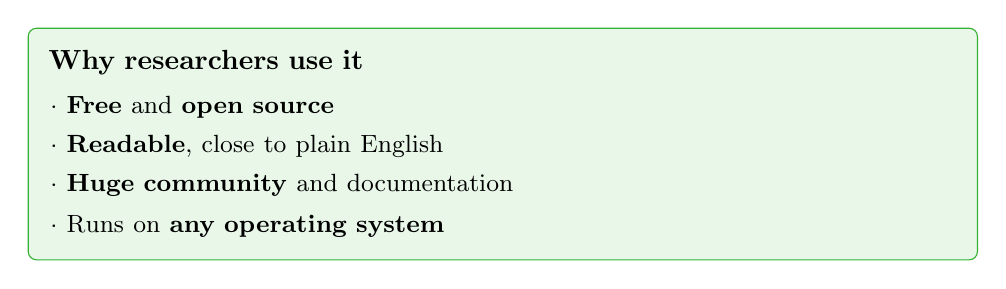
\begin{tikzpicture}
    \node[fill=lightgreen, draw=wurgreen, rounded corners=3pt,
          inner xsep=8pt, inner ysep=8pt, text width=\columnwidth-18pt]{%
      \textbf{Why researchers use it}\\[5pt]
      {\small
      $\cdot$ \textbf{Free} and \textbf{open source}\\[3pt]
      $\cdot$ \textbf{Readable}, close to plain English\\[3pt]
      $\cdot$ \textbf{Huge community} and documentation\\[3pt]
      $\cdot$ Runs on \textbf{any operating system}}};
  \end{tikzpicture}

  \column{0.48\textwidth}
  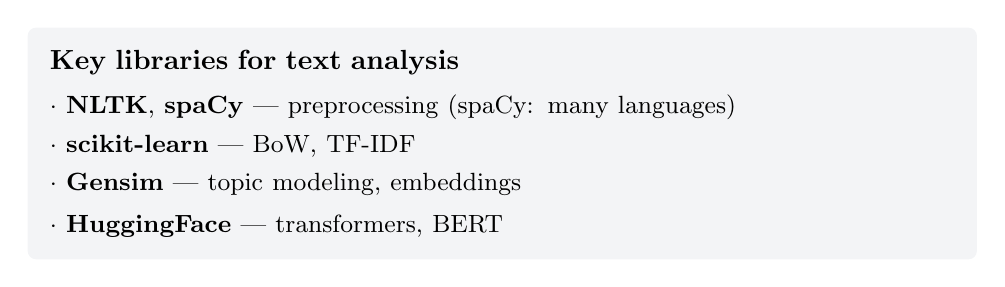
\begin{tikzpicture}
    \node[fill=lightgray, rounded corners=3pt,
          inner xsep=8pt, inner ysep=8pt, text width=\columnwidth-18pt]{%
      \textbf{Key libraries for text analysis}\\[5pt]
      {\small
      $\cdot$ \textbf{NLTK}, \textbf{spaCy} --- preprocessing (spaCy: many languages)\\[3pt]
      $\cdot$ \textbf{scikit-learn} --- BoW, TF-IDF\\[3pt]
      $\cdot$ \textbf{Gensim} --- topic modeling, embeddings\\[3pt]
      $\cdot$ \textbf{HuggingFace} --- transformers, BERT}};
  \end{tikzpicture}
\end{columns}
\end{frame}

% ── SLIDE 2: Why Python? ─────────────────────────────────────────────────────
\begin{frame}{Python vs.\ R}
\vspace{0.3cm}
{\small\textcolor{midgray}{\textit{Many of you probably already know R. Both are valid --- here is how they compare for this kind of work.}}}

\bigskip
\begin{columns}[t]
  \column{0.48\textwidth}
  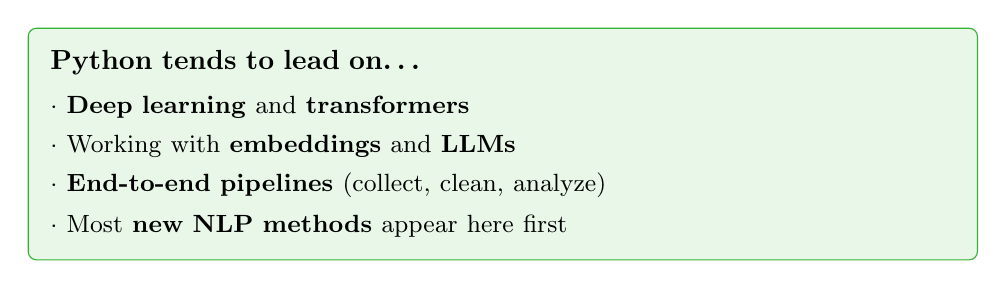
\begin{tikzpicture}
    \node[fill=lightgreen, draw=wurgreen, rounded corners=3pt,
          inner xsep=8pt, inner ysep=8pt, text width=\columnwidth-18pt]{%
      \textbf{Python tends to lead on\ldots}\\[5pt]
      {\small
      $\cdot$ \textbf{Deep learning} and \textbf{transformers}\\[3pt]
      $\cdot$ Working with \textbf{embeddings} and \textbf{LLMs}\\[3pt]
      $\cdot$ \textbf{End-to-end pipelines} (collect, clean, analyze)\\[3pt]
      $\cdot$ Most \textbf{new NLP methods} appear here first}};
  \end{tikzpicture}

  \column{0.48\textwidth}
  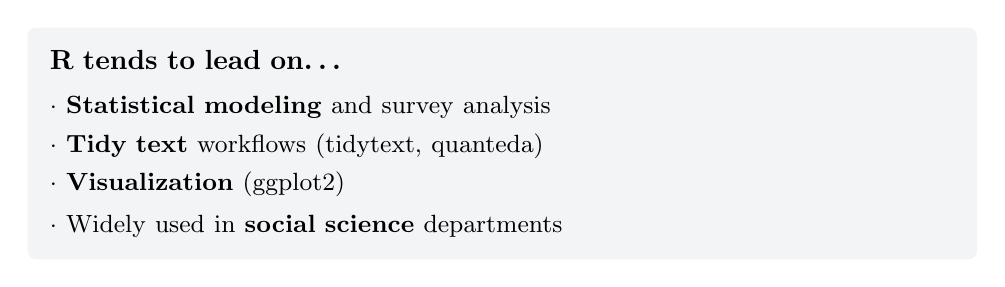
\begin{tikzpicture}
    \node[fill=lightgray, rounded corners=3pt,
          inner xsep=8pt, inner ysep=8pt, text width=\columnwidth-18pt]{%
      \textbf{R tends to lead on\ldots}\\[5pt]
      {\small
      $\cdot$ \textbf{Statistical modeling} and survey analysis\\[3pt]
      $\cdot$ \textbf{Tidy text} workflows (tidytext, quanteda)\\[3pt]
      $\cdot$ \textbf{Visualization} (ggplot2)\\[3pt]
      $\cdot$ Widely used in \textbf{social science} departments}};
  \end{tikzpicture}
\end{columns}

\bigskip
{\small If you know R, Python will feel familiar quickly. This course uses Python,
but the concepts transfer.}
\end{frame}

% ── SLIDE 3: What is Colab? ──────────────────────────────────────────────────
\begin{frame}{What is Google Colab?}
\vspace{0.2cm}
{\small Google Colab is a \textbf{free, browser-based environment} for writing and running
Python code. \textbf{No installation needed} --- you open a link and start coding.
Everything runs on \textbf{Google's servers}, not your own machine.
It uses the \textbf{notebook format}: code cells you run one at a time,
mixed with text cells for notes. Great for teaching, and for keeping
analysis \textbf{readable and reproducible}.}

\bigskip
\begin{columns}[t]
  \column{0.48\textwidth}
  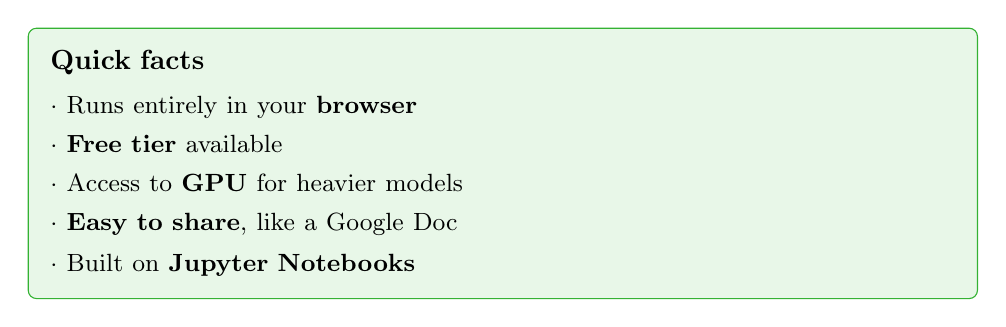
\begin{tikzpicture}
    \node[fill=lightgreen, draw=wurgreen, rounded corners=3pt,
          inner xsep=8pt, inner ysep=8pt, text width=\columnwidth-18pt]{%
      \textbf{Quick facts}\\[5pt]
      {\small
      $\cdot$ Runs entirely in your \textbf{browser}\\[3pt]
      $\cdot$ \textbf{Free tier} available\\[3pt]
      $\cdot$ Access to \textbf{GPU} for heavier models\\[3pt]
      $\cdot$ \textbf{Easy to share}, like a Google Doc\\[3pt]
      $\cdot$ Built on \textbf{Jupyter Notebooks}}};
  \end{tikzpicture}

  \column{0.48\textwidth}
  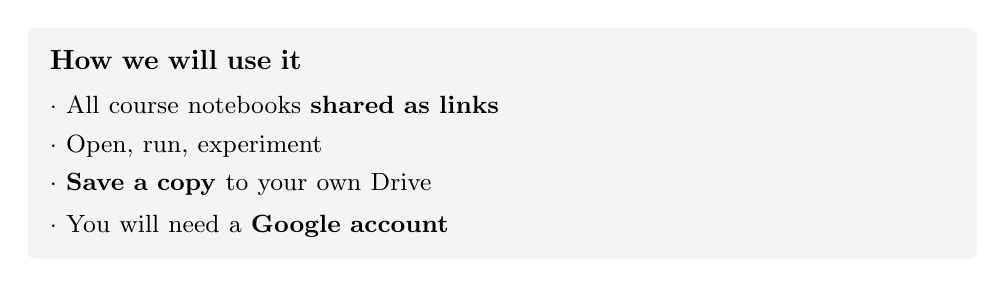
\begin{tikzpicture}
    \node[fill=lightgray, rounded corners=3pt,
          inner xsep=8pt, inner ysep=8pt, text width=\columnwidth-18pt]{%
      \textbf{How we will use it}\\[5pt]
      {\small
      $\cdot$ All course notebooks \textbf{shared as links}\\[3pt]
      $\cdot$ Open, run, experiment\\[3pt]
      $\cdot$ \textbf{Save a copy} to your own Drive\\[3pt]
      $\cdot$ You will need a \textbf{Google account}}};
  \end{tikzpicture}
\end{columns}
\end{frame}

% ── SLIDE 4: Colab pros and cons ─────────────────────────────────────────────
\begin{frame}{Colab: Pros and Cons}
\vspace{0.3cm}
\begin{columns}[t]
  \column{0.48\textwidth}
  \begin{tikzpicture}
    \node[fill=lightgreen, draw=wurgreen, rounded corners=3pt,
          inner xsep=8pt, inner ysep=8pt, text width=\columnwidth-18pt]{%
      \textcolor{darkgreen}{\textbf{\faThumbsUp\enspace Pros}}\\[6pt]
      {\small
      $\cdot$ \textbf{Zero setup}, works out of the box\\[3pt]
      $\cdot$ \textbf{Same environment} for everyone\\[3pt]
      $\cdot$ Free \textbf{GPU access} for heavier models\\[3pt]
      $\cdot$ Easy to \textbf{share and collaborate}\\[3pt]
      $\cdot$ All course materials in \textbf{one link}\\[3pt]
      $\cdot$ \textbf{Saves automatically} to Google Drive}};
  \end{tikzpicture}

  \column{0.48\textwidth}
  \begin{tikzpicture}
    \node[fill=warnred, draw=warnborder, rounded corners=3pt,
          inner xsep=8pt, inner ysep=8pt, text width=\columnwidth-18pt]{%
      \textcolor{warnborder}{\textbf{\faThumbsDown\enspace Cons}}\\[6pt]
      {\small
      $\cdot$ Needs a \textbf{stable internet} connection\\[3pt]
      $\cdot$ Sessions \textbf{time out} after inactivity\\[3pt]
      $\cdot$ Free tier has \textbf{usage limits}\\[3pt]
      $\cdot$ Not great for \textbf{very large datasets}\\[3pt]
      $\cdot$ \textbf{Data privacy} considerations (Google)\\[3pt]
      $\cdot$ \textbf{Less control} than a local environment}};
  \end{tikzpicture}
\end{columns}

\medskip
{\small\textcolor{midgray}{\textit{For this course, the pros far outweigh the cons.
Once you are comfortable, setting up a local environment is a natural next step.}}}
\end{frame}

\end{document}
